\subsection{UC 6.1.2: Edit}
		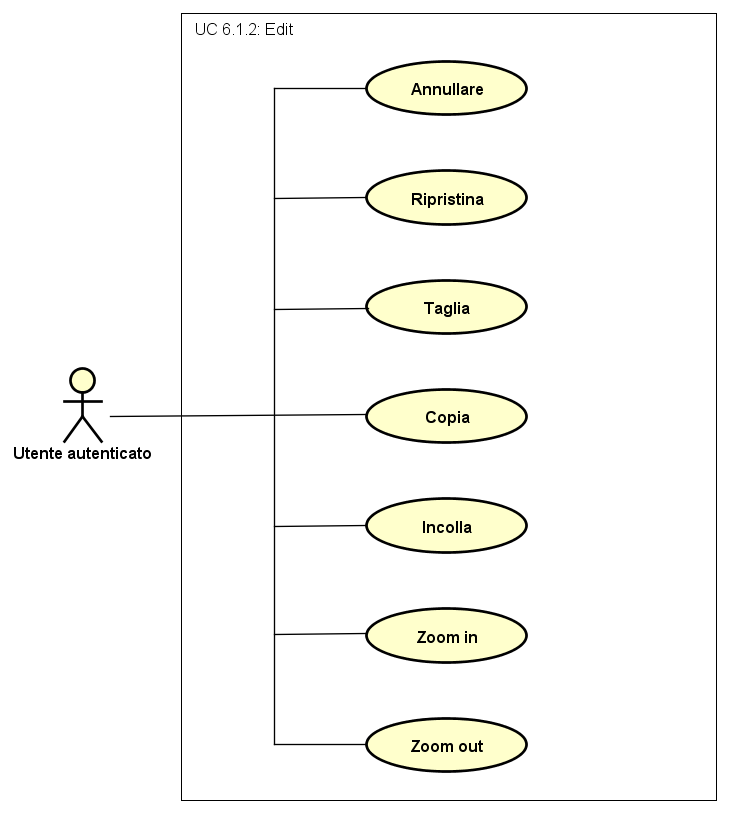
\includegraphics[scale=0.7]{../../Casi D'uso/UC 6.1.2.png}
\begin{itemize}
		\item \textbf{Attori coinvolti:} Utente autenticato. \\
		\item \textbf{Scopo e descrizione:} L'utente autenticato può accedere alle voci undo, redo, cut, copy, paste, zoom + e zoom - appartenenti alla voce edit del menù. \\
		\item \textbf{Precondizione:} L'applicazione offre all'utente la voce edit appartenente barra dei menù. \\
		\item \textbf{Postcondizione:} L'applicazione, a seconda dell'operazione richiesta dall'utente, effettua la modifica. \\
\end{itemize}